\setcounter{num}{0}
\setcounter{numz}{0}
\begin{tcolorbox}[colframe=GKD,colback=white,coltitle=white,title=Allgemeines:\indent Körperwaffen\indent {\scriptsize \textcopyright\,Roland Habersetzer - Die Grundtechniken des Karate - Auszüge}]
	\null\vfill\null	
	\begin{tabularx}{\textwidth}{cccc}
		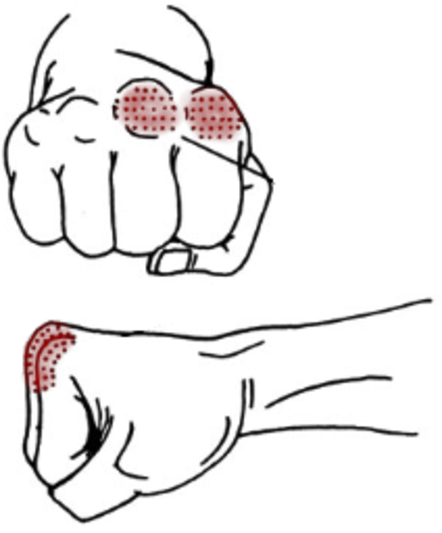
\includegraphics[height=0.12\textwidth-2\tabcolsep,keepaspectratio]{habersetzer_waffen_hand_seiken}	& 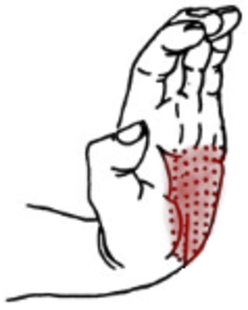
\includegraphics[height=0.12\textwidth-2\tabcolsep,keepaspectratio]{habersetzer_waffen_hand_teisho}	& 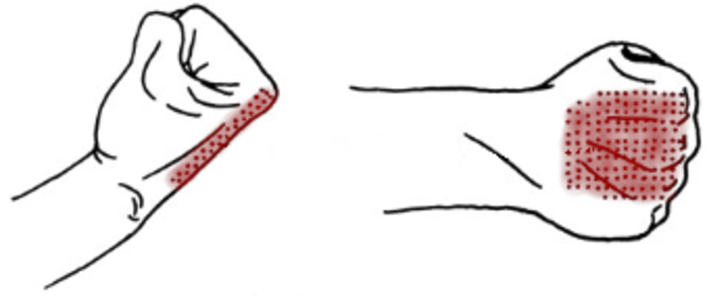
\includegraphics[height=0.12\textwidth-2\tabcolsep,keepaspectratio]{habersetzer_waffen_hand_uraken}	& 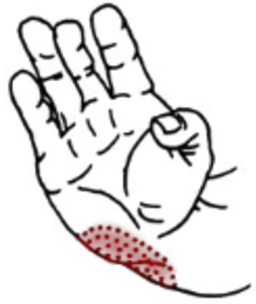
\includegraphics[height=0.12\textwidth-2\tabcolsep,keepaspectratio]{habersetzer_waffen_hand_seiryuto} \\
		Seiken 	& Teisho 	& Uraken 	& Seiryuto\\
		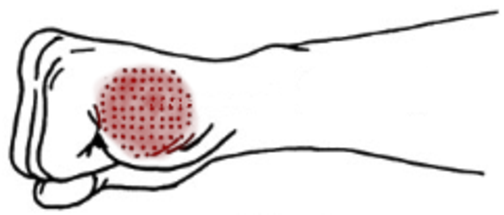
\includegraphics[height=0.12\textwidth-2\tabcolsep,keepaspectratio]{habersetzer_waffen_hand_tettsui} & 
\includegraphics[height=0.12\textwidth-2\tabcolsep,keepaspectratio]{habersetzer_waffen_hand_nakadaka_ippon_ken} & 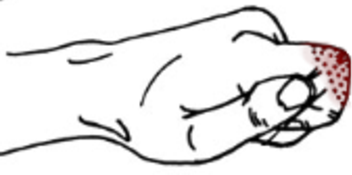
\includegraphics[height=0.12\textwidth-2\tabcolsep,keepaspectratio]{habersetzer_waffen_hand_ippon_ken} & 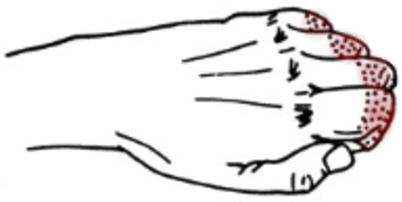
\includegraphics[height=0.12\textwidth-2\tabcolsep,keepaspectratio]{habersetzer_waffen_hand_hiraken} \\
		Tettsui 	& Nakadaka 	& Ippon Ken & Hiraken \\
		
\includegraphics[height=0.12\textwidth-2\tabcolsep,keepaspectratio]{habersetzer_waffen_hand_haito} & 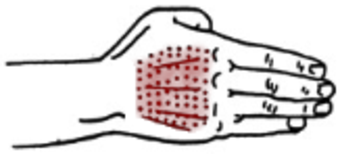
\includegraphics[height=0.12\textwidth-2\tabcolsep,keepaspectratio]{habersetzer_waffen_hand_haishu}	& 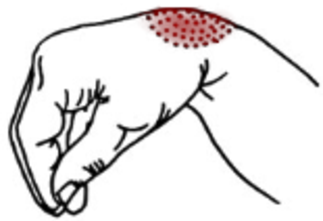
\includegraphics[height=0.12\textwidth-2\tabcolsep,keepaspectratio]{habersetzer_waffen_hand_koken} & 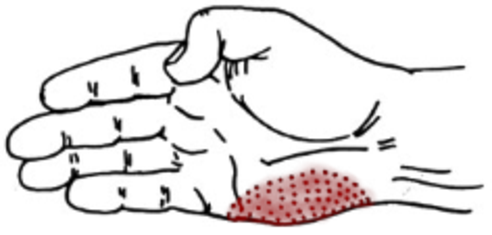
\includegraphics[height=0.12\textwidth-2\tabcolsep,keepaspectratio]{habersetzer_waffen_hand_shuto} \\
		Haito 	& Haishu 	& Koken 		& Shuto \\	
		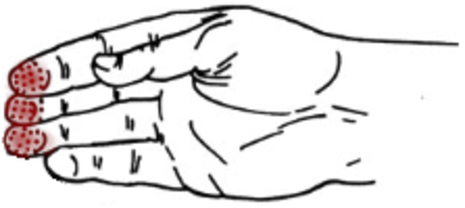
\includegraphics[height=0.12\textwidth-2\tabcolsep,keepaspectratio]{habersetzer_waffen_hand_nukite}	& 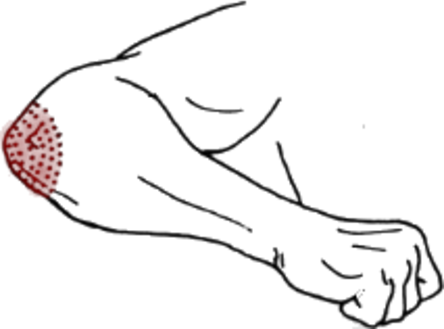
\includegraphics[height=0.12\textwidth-2\tabcolsep,keepaspectratio]{habersetzer_waffen_hand_empi} & 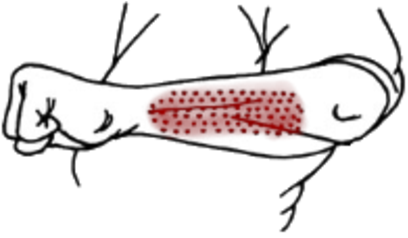
\includegraphics[height=0.12\textwidth-2\tabcolsep,keepaspectratio]{habersetzer_waffen_hand_wan} & \\
		Nukite 	& Empi 		& Wan 			& \\
	\end{tabularx}\\
	%\freefootnote{\textcopyright\,Roland Habersetzer - Die Grundtechniken des Karate}\\
	\null\vfill\null
	
\end{tcolorbox}
%%------------------------------------------------------------------------------
\clearpage
\pagebreak
%%------------------------------------------------------------------------------
\setcounter{num}{0}
\setcounter{numz}{0}
\begin{tcolorbox}[colframe=GKD,colback=white,coltitle=white,title=Allgemeines:\indent Körperwaffen\indent {\scriptsize \textcopyright\,Roland Habersetzer - Die Grundtechniken des Karate - Auszüge}]
	\null\vfill\null	
	\begin{tabularx}{\textwidth}{cccc}
		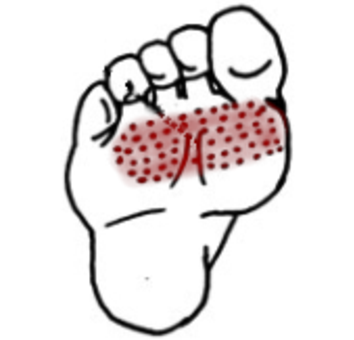
\includegraphics[height=0.18\textwidth-2\tabcolsep,keepaspectratio]{habersetzer_waffen_fuss_koshi} 		& 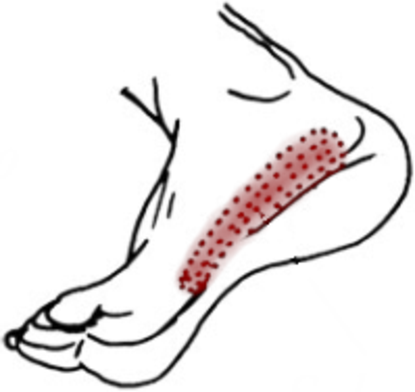
\includegraphics[height=0.18\textwidth-2\tabcolsep,keepaspectratio]{habersetzer_waffen_fuss_sokuto} 		& 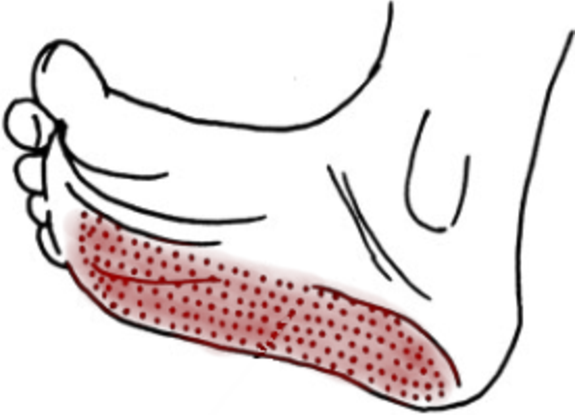
\includegraphics[height=0.18\textwidth-2\tabcolsep,keepaspectratio]{habersetzer_waffen_fuss_teisoku} &
		\multirow{3}{*}{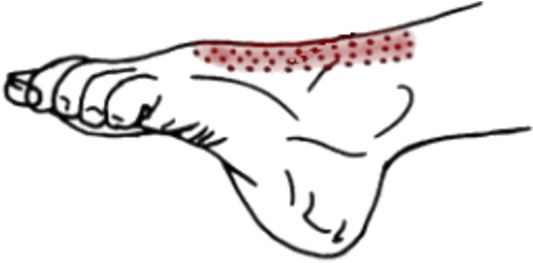
\includegraphics[height=0.18\textwidth-2\tabcolsep,keepaspectratio]{habersetzer_waffen_fuss_haisoku}}
		\\
		Koshi 		& Sokuto 	& Teisoku &\\
		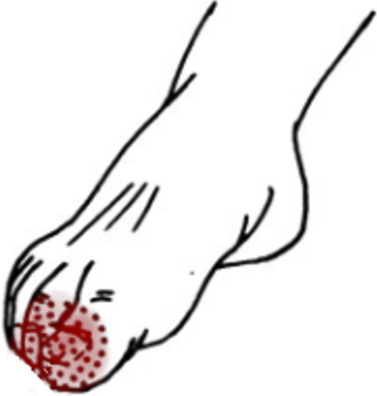
\includegraphics[height=0.18\textwidth-2\tabcolsep,keepaspectratio]{habersetzer_waffen_fuss_tsumasaki} 	& 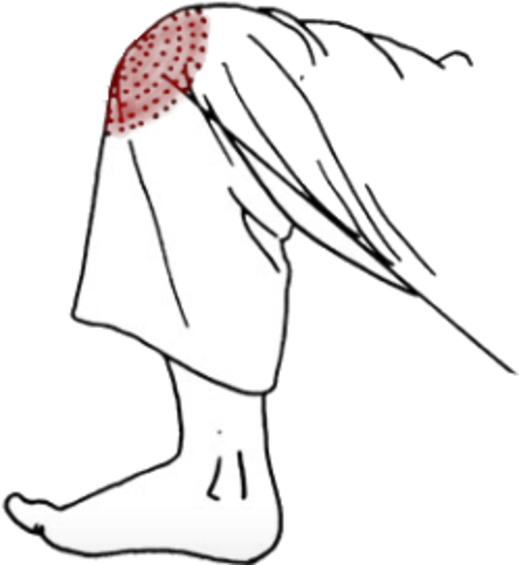
\includegraphics[height=0.18\textwidth-2\tabcolsep,keepaspectratio]{habersetzer_waffen_fuss_hiza} 		&  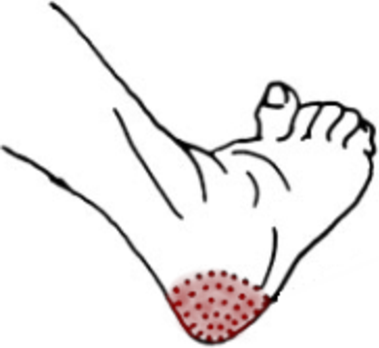
\includegraphics[height=0.18\textwidth-2\tabcolsep,keepaspectratio]{habersetzer_waffen_fuss_kakato} &\\
		Tsumasaki 	& Hiza 		& Kakato & Haisoku\\
	\end{tabularx}
	%\null\vfill\null
	%\freefootnote{\textcopyright\,Roland Habersetzer - Die Grundtechniken des Karate}
	\null\vfill\null
\end{tcolorbox}
%%------------------------------------------------------------------------------
\clearpage
\pagebreak
%%------------------------------------------------------------------------------
\begin{tcolorbox}[colframe=GKD,colback=white,coltitle=white,title=Allgemeines:\indent Grundlegende Dachi Waza]
	\null\vfill\null
	\setcounter{num}{0}
	\setcounter{numz}{0}	
	\begin{tabularx}{\textwidth}{cccc}
		
\includegraphics[width=0.25\textwidth-2\tabcolsep,keepaspectratio]{musubi_dachi.pdf}	&
		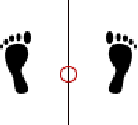
\includegraphics[width=0.25\textwidth-2\tabcolsep,keepaspectratio]{heiko_dachi.pdf} &
		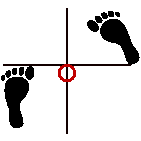
\includegraphics[width=0.25\textwidth-2\tabcolsep,keepaspectratio]{sanchin_dachi.pdf} & \\
		Musubi Dachi 		& Heiko Dachi 	& Sanchin Dachi & \\
		
\includegraphics[width=0.25\textwidth-2\tabcolsep,keepaspectratio]{nekoashi_dachi.pdf} & \multicolumn{2}{c}{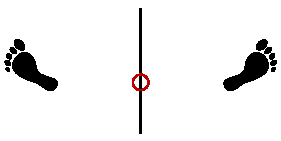
\includegraphics[width=0.5\textwidth-1\tabcolsep,keepaspectratio]{shiko_dachi.pdf}} & \multirow[t]{3}{*}{
\includegraphics[width=0.25\textwidth-2\tabcolsep,keepaspectratio]{zenkutsu_dachi.pdf}}\\
		Neko-Ashi Dachi 	& \multicolumn{2}{c}{Shiko Dachi} 	& Zenkutsu Dachi  \\							
	\end{tabularx}\\\null\vfill\null
\end{tcolorbox}
%%------------------------------------------------------------------------------
\clearpage
\pagebreak
%%------------------------------------------------------------------------------
